\documentclass[a4paper]{article}
\linespread{1.6}
\usepackage{geometry}
\usepackage{setspace}
\usepackage{amsmath}
\usepackage{amssymb}
\usepackage{enumerate}
\usepackage{subfigure}
\usepackage{caption}
\usepackage{listings}
\usepackage{float}
\captionsetup{font = footnotesize}
\usepackage[pdftex]{graphicx}
\geometry{left=1cm,right=1cm,top=2.5cm,bottom=2.5cm}

\begin{document}
\begin{spacing}{2.0}
\begin{flushleft}\begin{huge}EEE6561  Fundamentals of Biometric Identification   Homework 3\end{huge}
\end{flushleft}
\begin{flushright}\begin{Large}Hudanyun Sheng\end{Large}\end{flushright}
\section*{\huge\textbf{ Part \uppercase\expandafter{\romannumeral1} Entire Face Performance}  }
	\normalsize
	\begin{enumerate}[(a)]
	\item Plot the genuine and impostor score distributions.
	\item Plot the Cumulative Match Characteristic curves.
	\item Plot the Receiver Operating Curve (FAR vs. FRR).
	\end{enumerate}
	
	The genuine and the imposter score distributions (part (a)) are shown in same graph as histograms of 	the  score distributions with 100 bins for each of them, shown in the form of probability, in figure 		\ref{scoreDis}; the cumulative match characteristic curve(part (b)) is shown in figure \ref{CMC}; the 		receiver operating curve (FAR vs. FRR, part (c)) is shown in figure \ref{ROC}.
	
	\begin{figure}[h]
	\begin{minipage}[t]{0.3\linewidth}
	\centering
	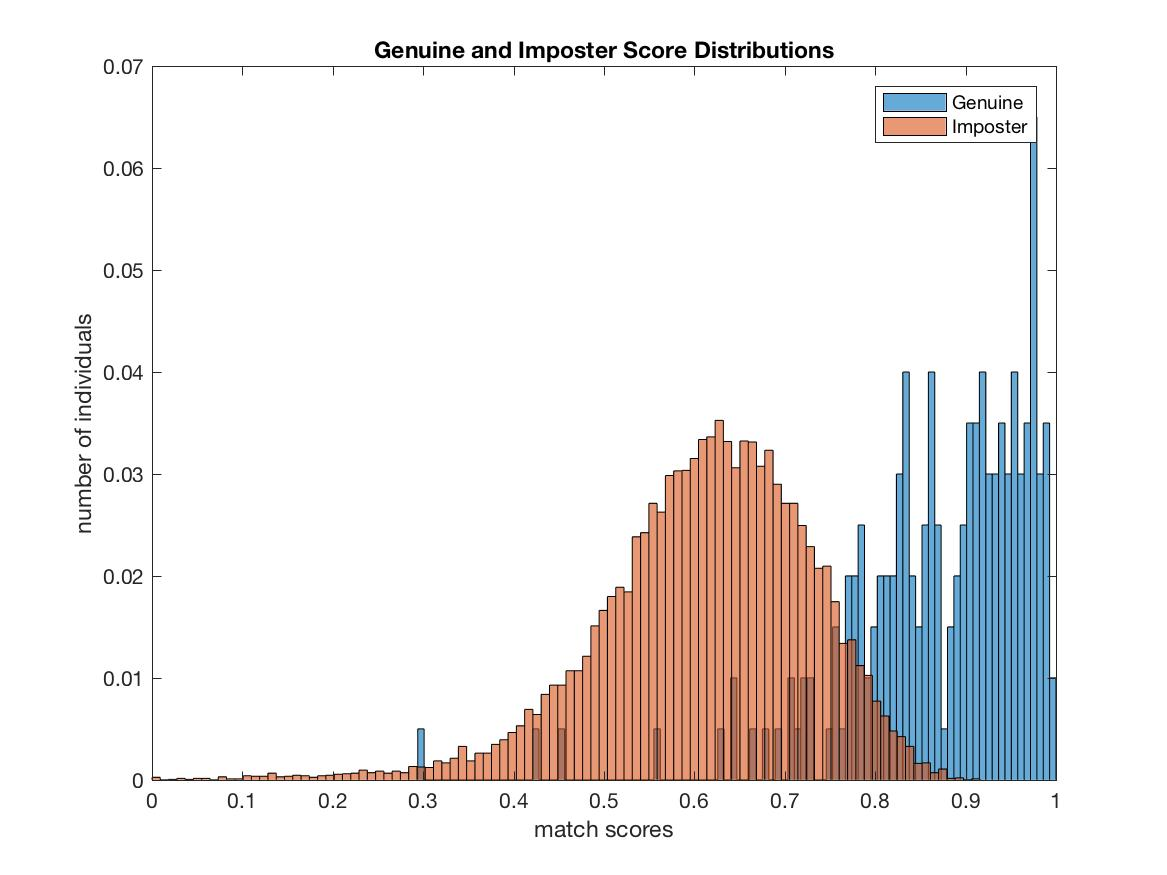
\includegraphics[width = 2.4in]{AllscoreDis.jpg}
	\caption{The genuine and imposter score distributions.}
	\label{scoreDis}
	\end{minipage}
	\begin{minipage}[t]{0.3\linewidth}
	\centering
	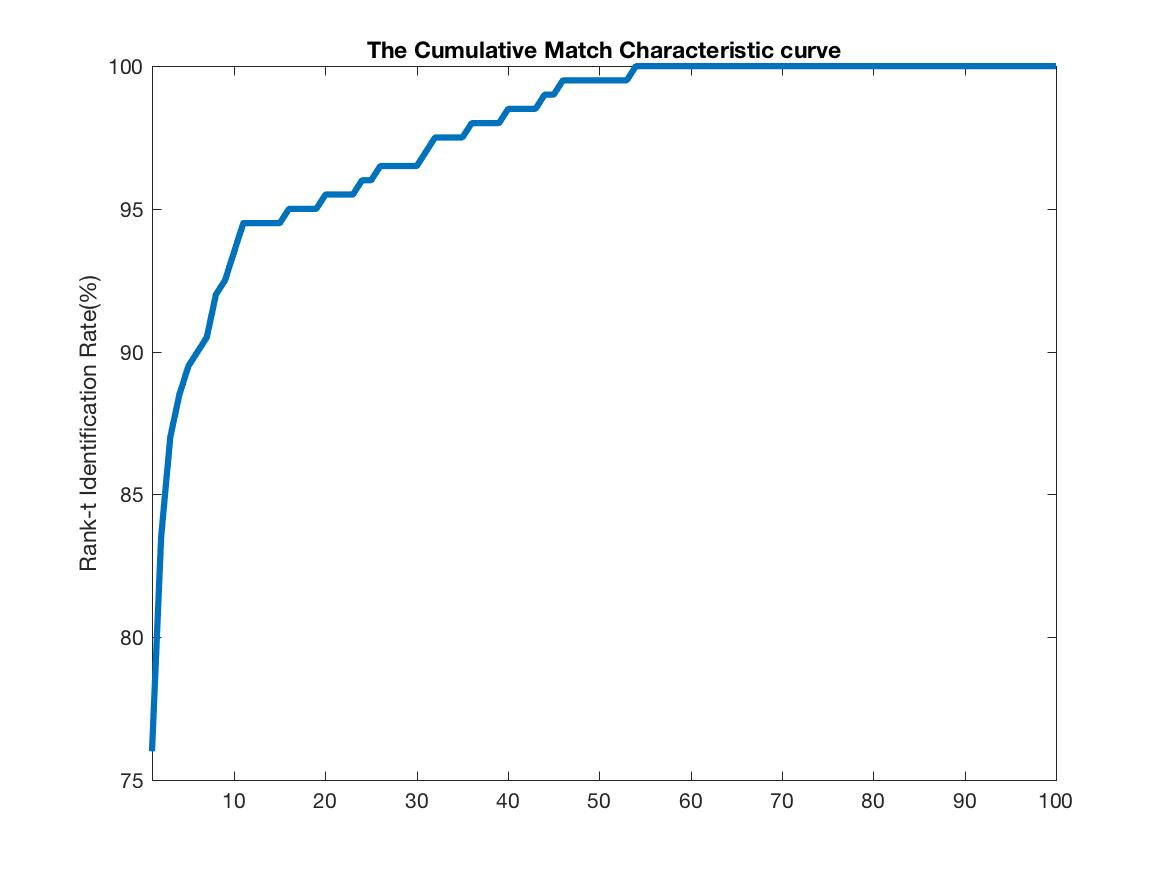
\includegraphics[width = 2.4in]{AllCMC.jpg}
	\caption{The Cumulative Match Characteristic curves}
	\label{CMC}
	\end{minipage}
	\begin{minipage}[t]{0.3\linewidth}
	\centering
	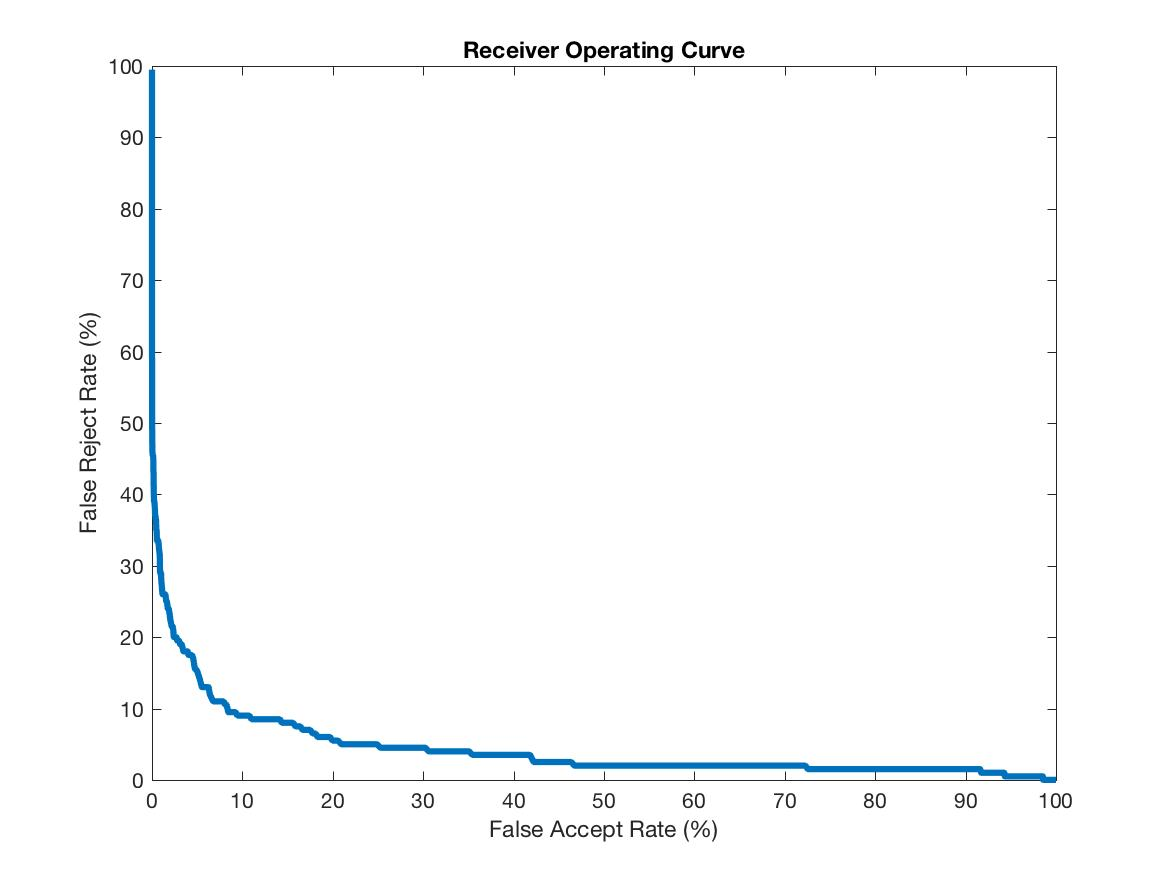
\includegraphics[width = 2.4in]{AllROC.jpg}
	\caption{The Receiver Operating curve}
	\label{ROC}
	\end{minipage}
	\end{figure}



	

\section*{\huge\textbf{ Part \uppercase\expandafter{\romannumeral2} Partial Face Performance}  }
	\normalsize
	Different parts of the face contain varying amounts of discriminating power. Using only the top half, bottom half, left half, and right half of the facial images to:
	\begin{enumerate}[(a)]
	\item Plot the genuine and impostor score distributions.
	\item Plot the Cumulative Match Characteristic curves.
	\item Plot the Receiver Operating Curve (FAR vs. FRR).
	\end{enumerate}
	
	Are any of the performance numbers of the partial face experiments close to those obtained when using the entire face image? Which of the partial face regions perform the best? Are the perfor- mance numbers obtained using the partial face expected?(Why or why not?) Providing sufficient detail, how could the performance numbers of the entire face based system be improved using those obtained from partial face experiments?\\
	
	The genuine and the imposter score distributions (part (a)) are shown in same graph as histograms of 	the  score distributions with 100 bins for each of them, shown in the form of probability, in figures 		\ref{scoreDisTop}, \ref{scoreDisBottom}, \ref{scoreDisLeft}, \ref{scoreDisRight}. The comparisons of the Cumulative Match Characteristic curves and the Receiver Operating Curve are shown in figure 	\ref{cmcCom} and figure \ref{rocCom} respectively. The comparison of several performance measure, i.e. d-prime value, rank-1 identification rate and rank-10 identification rate, are summarized and shown in table \ref{comTable}.
	
	\begin{figure}[!htb]
	\begin{minipage}[t]{0.5\linewidth}
	\centering
	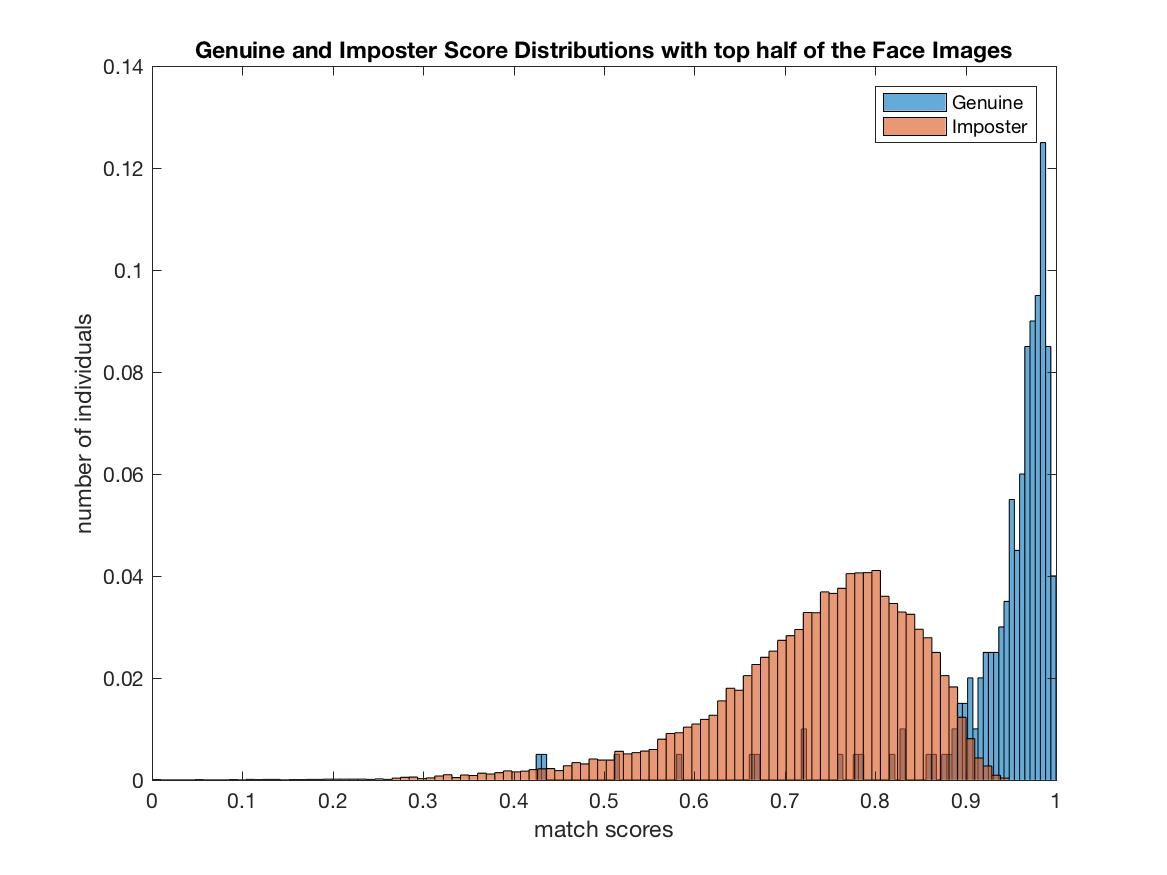
\includegraphics[width = 3.5in]{top_scoreDis.jpg}
	\caption{The genuine and imposter score distributions when only top half of the facial images are used.}
	\label{scoreDisTop}
	\end{minipage}
	\begin{minipage}[t]{0.5\linewidth}
	\centering
	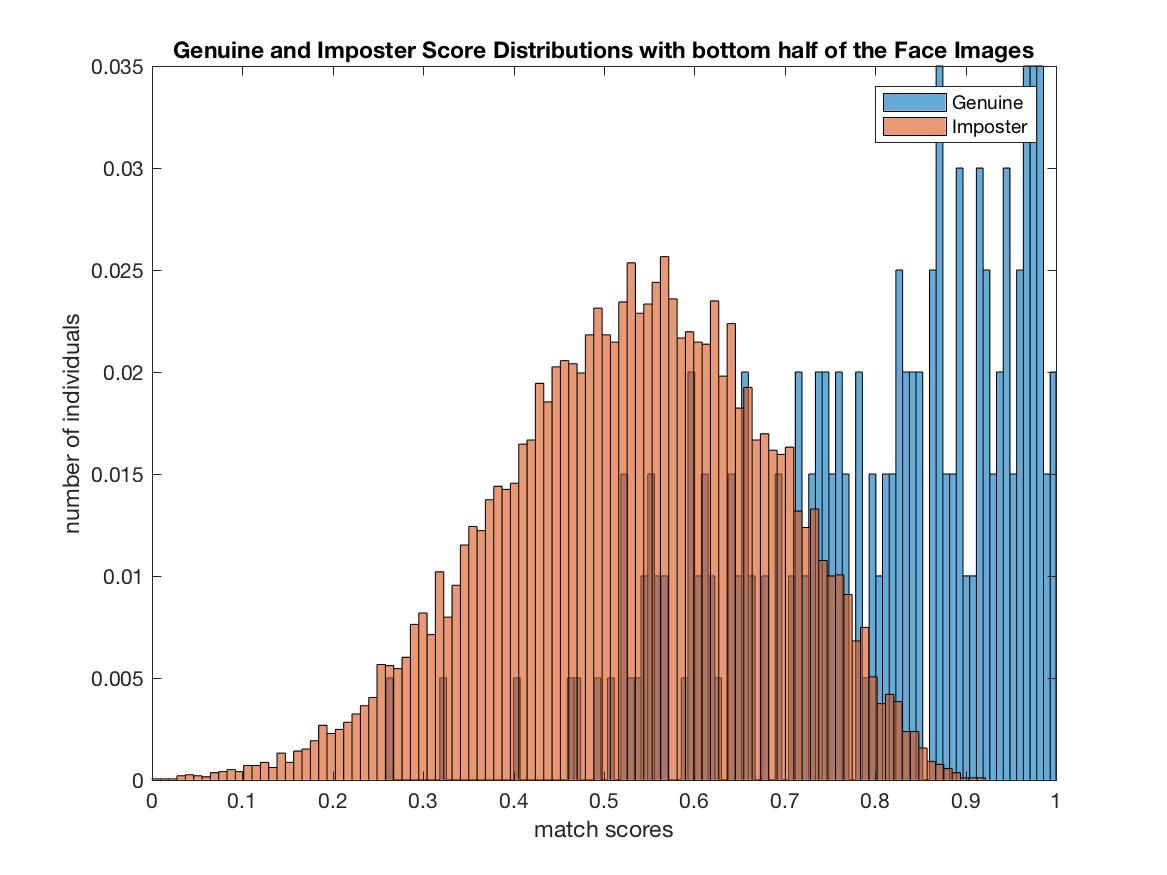
\includegraphics[width = 3.5in]{bottom_scoreDis.jpg}
	\caption{The genuine and imposter score distributions when only bottom half of the facial images are used.}
	\label{scoreDisBottom}
	\end{minipage}
	\end{figure}	
	
	\begin{figure}[!htb]
	\begin{minipage}[t]{0.5\linewidth}
	\centering
	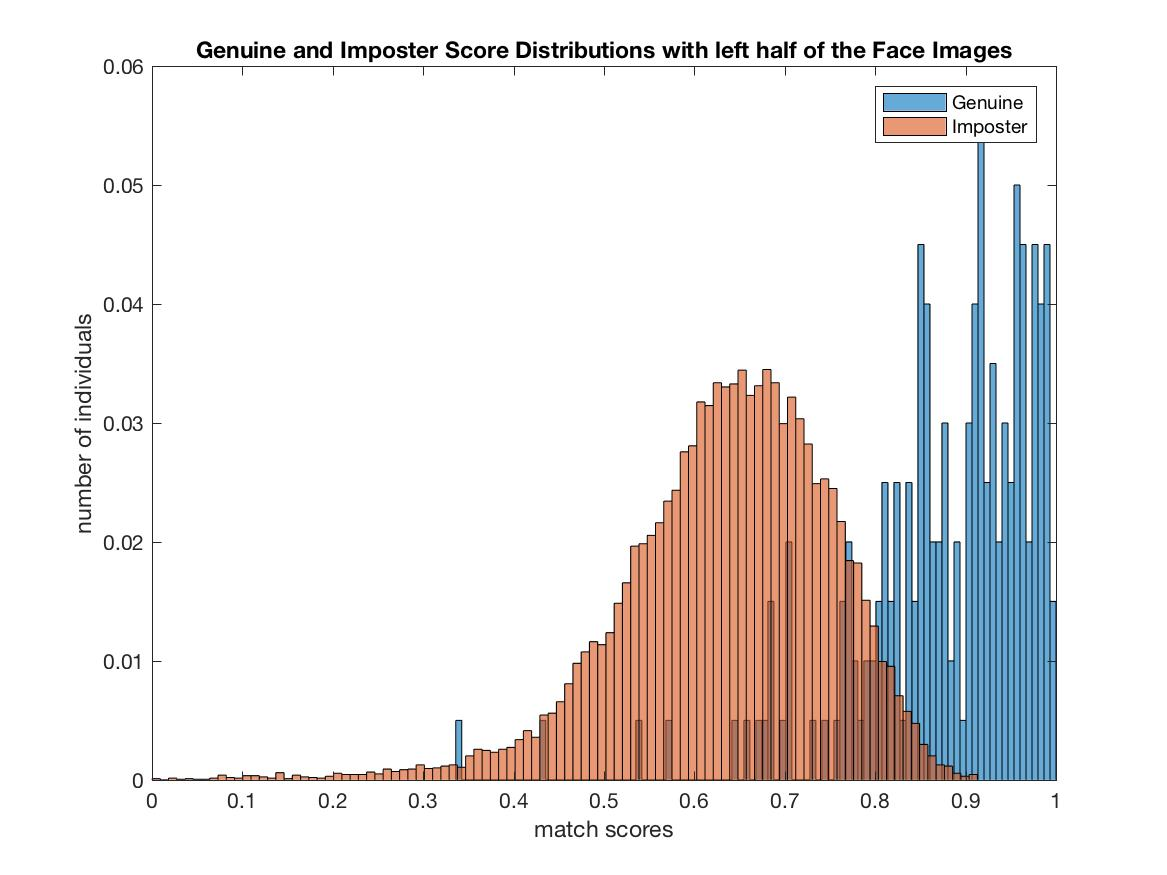
\includegraphics[width = 3.5in]{left_scoreDis.jpg}
	\caption{The genuine and imposter score distributions when only left half of the facial images are used.}
	\label{scoreDisLeft}
	\end{minipage}
	\begin{minipage}[t]{0.5\linewidth}
	\centering
	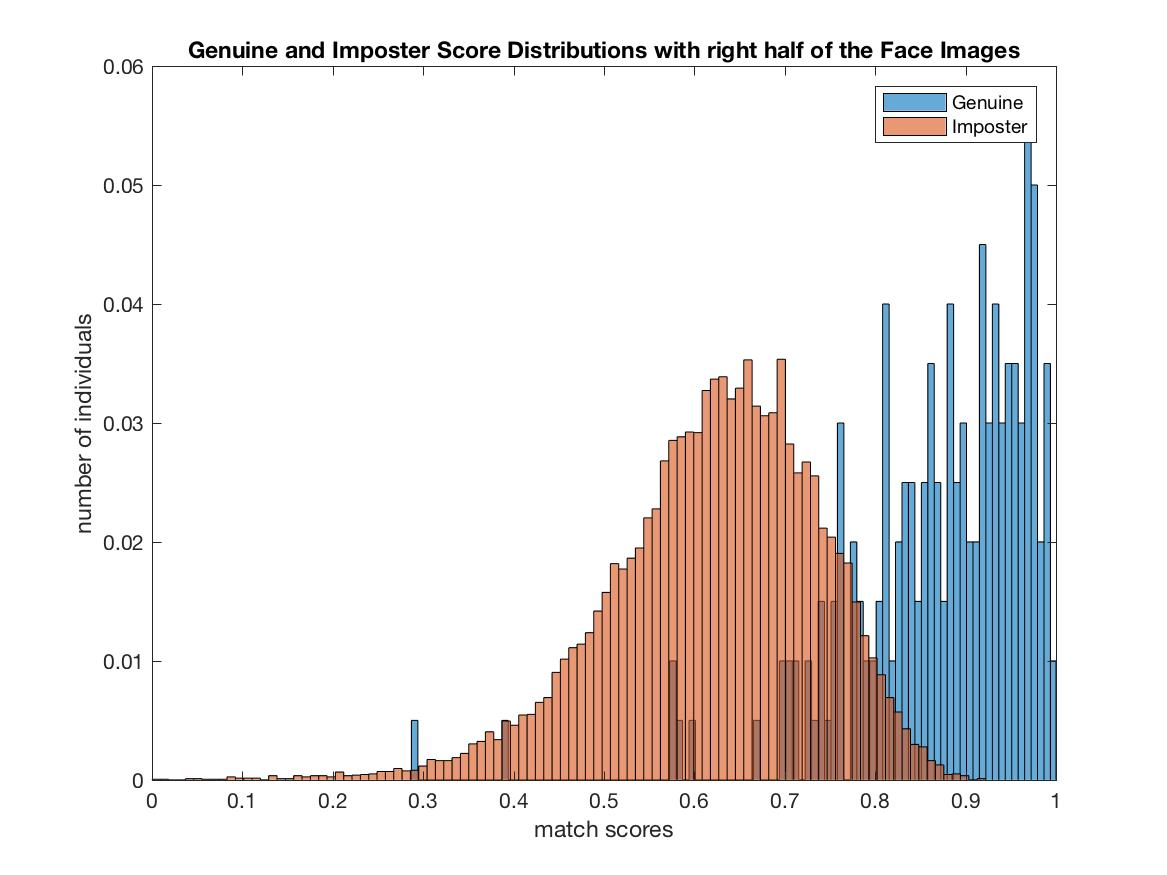
\includegraphics[width = 3.5in]{right_scoreDis.jpg}
	\caption{The genuine and imposter score distributions when only right half of the facial images are used.}
	\label{scoreDisRight}
	\end{minipage}
	\end{figure}	
	
	\begin{figure}[!htb]
	\begin{minipage}[t]{0.5\linewidth}
	\centering
	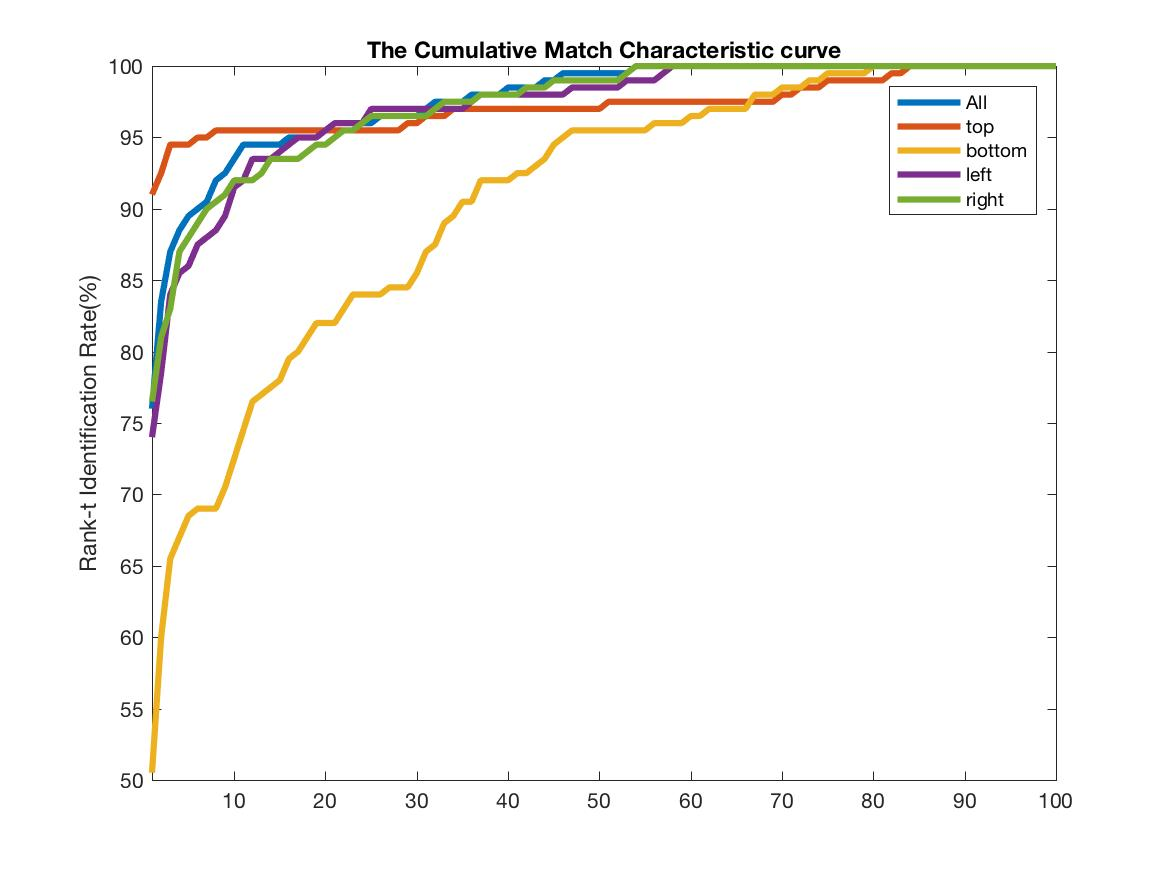
\includegraphics[width = 3.5in]{inoneCMC.jpg}
	\caption{The comparison of the Cumulative Match Characteristic curve when using whole face, top, bottom, left and right half of the face images.}
	\label{cmcCom}
	\end{minipage}
	\begin{minipage}[t]{0.5\linewidth}
	\centering
	\includegraphics[width = 3.5in]{inoneROC.jpg}
	\caption{The comparison of the Receiver Operating Characteristic curve when using whole face, top, bottom, left and right half of the face images.}
	\label{rocCom}
	\end{minipage}
	\end{figure}	
	
	\begin{table}[!htb]
	\centering  
	\begin{tabular}{lccc}  
	\hline
	Part of face image & $d'$ value & rank-1 identification rate & rank-10 identification rate\\ \hline  
	entire & 2.3339 & $76.0\%$ & $93.5\%$\\         
	top & 2.0589 & $91.0\%$ & $95.5\%$\\      
	bottom &1.7667 & $50.5\%$ & $72.5\%$\\ 
	left &2.2246 & $74.0\%$ & $91.5\%$\\ 
	right &2.2599 & $76.5\%$ & $92.\%$\\ \hline
	\end{tabular}
	\caption{Comparison of some performance measures}
	\label{comTable}
	\end{table}
	
	Based on the plots and tables shown above, it is easy to analyze and conclude that by using the top, left or right half of the face images, similar performances are able to be obtained when using the entire face image. But by using only bottom half of the face images would get a bad performance. What is more, using only top half of the face images can even out-perform the performance of using the entire face images. As shown in the score distributions, we can  see that with only top half of the face images, the genuine and imposter scores are better separated compared to others, including one using the entire face image. The conclusion can also be drawn by examining the CMC curve, with a higher rank-one identification rate, as well as the ROC curve, which appears much closer to the axises. When looking at the d-prime value, we would see that using only top half of the face images, though seems to outperforms others concluded from the graphs, has a rather small d-prime value, which may result from the distribution not being normal. Which also makes us pay attention that we cannot rely on only one measurement to determine whether a system is good or not. Based on the plots and analysis above, top half of the face regions performs the best. This result is the same as I expected. As learned during class, the top half of the face is much more important compared to the bottom half, and nose is not import compared to eyes. The potential methods of improving the performance of the entire face based system can be using the image of whole face, with much weight put on the top half.


\newpage
\section*{\huge\textbf{Extra Credit: PCA Based Facial Recognition}}
	The plot showing the fraction of total variance retained with number of eigenvalues is shown in figure \ref{pca}. It is easy to conclude that with projection into a space of 61 dimension, $95\%$ of the total variance is retained. So I decided to keep 61 eigenvalues. 
	
	\begin{figure}[h]
	\centering
	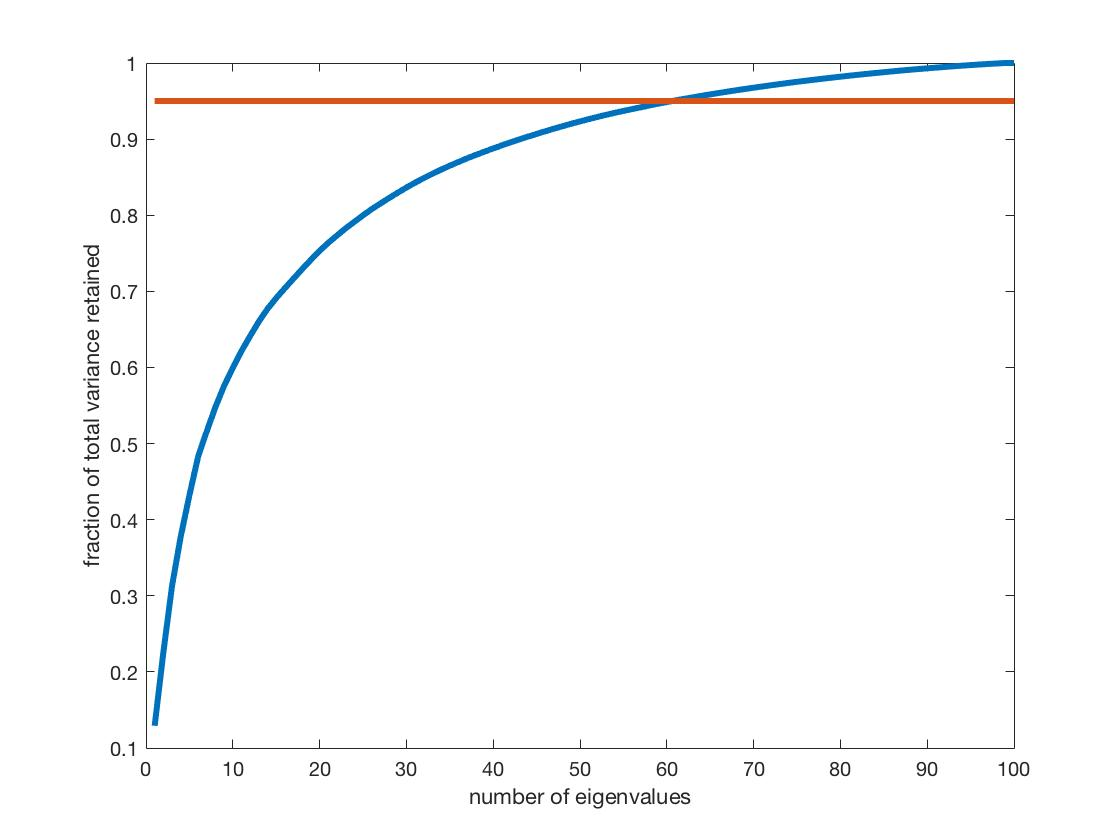
\includegraphics[width = 3.5in]{PCA.jpg}
	\caption{Plot of fraction of total variance retained vs. number of eigenvalues}
	\label{pca}
	\end{figure}
	
	The genuine and the imposter score distributions (part (a)) are shown in same graph as histograms of the score distrbutions with 100 bins for each of them, shown in the form of probability, in figure ; the cumulative match characteristic curve(part (b)) is shown in figure ; the receiver operating curve (FAR vs. FRR, part (c)) is shown in figure .
	
	\begin{figure}[h]
	\begin{minipage}[t]{0.3\linewidth}
	\centering
	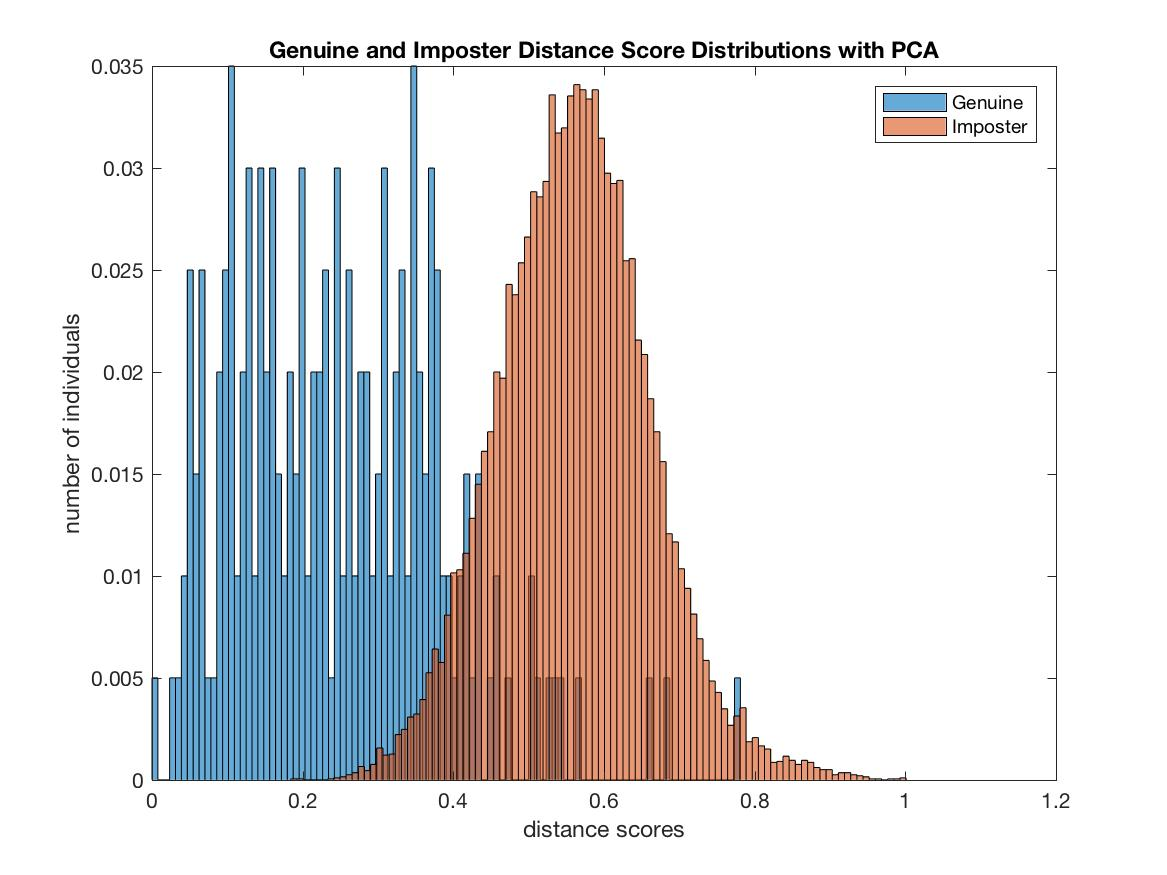
\includegraphics[width = 2.4in]{PCAallscoreDis.jpg}
	\caption{The genuine and imposter score distributions.}
	\label{scoreDispca}
	\end{minipage}
	\begin{minipage}[t]{0.3\linewidth}
	\centering
	\includegraphics[width = 2.4in]{pcaAllCMC.jpg}
	\caption{The Cumulative Match Characteristic curves}
	\label{CMCpca}
	\end{minipage}
	\begin{minipage}[t]{0.3\linewidth}
	\centering
	\includegraphics[width = 2.4in]{pcaAllROC.jpg}
	\caption{The Receiver Operating curve}
	\label{ROCpca}
	\end{minipage}
	\end{figure}

	If using only top, bottom, left, and right half of the face images, the genuine and the imposter score distributions (part (a)) are shown in same graph as histograms of the score distributions with 100 bins for each of them, shown in the form of probability, in figures \ref{scoreDisTopPCA}, \ref{scoreDisBottomPCA}, \ref{scoreDisLeftPCA}, \ref{scoreDisRightPCA}. The comparisons of the Cumulative Match Characteristic curves and the Receiver Operating Curve are shown in figure \ref{cmcComPCA} and figure \ref{rocComPCA} respectively. The comparison of several performance measure, i.e. d-prime value, rank-1 identification rate and rank-10 identification rate, are summarized and shown in table \ref{comTablePCA}.
	
	\begin{figure}[h!]
	\begin{minipage}[t]{0.5\linewidth}
	\centering
	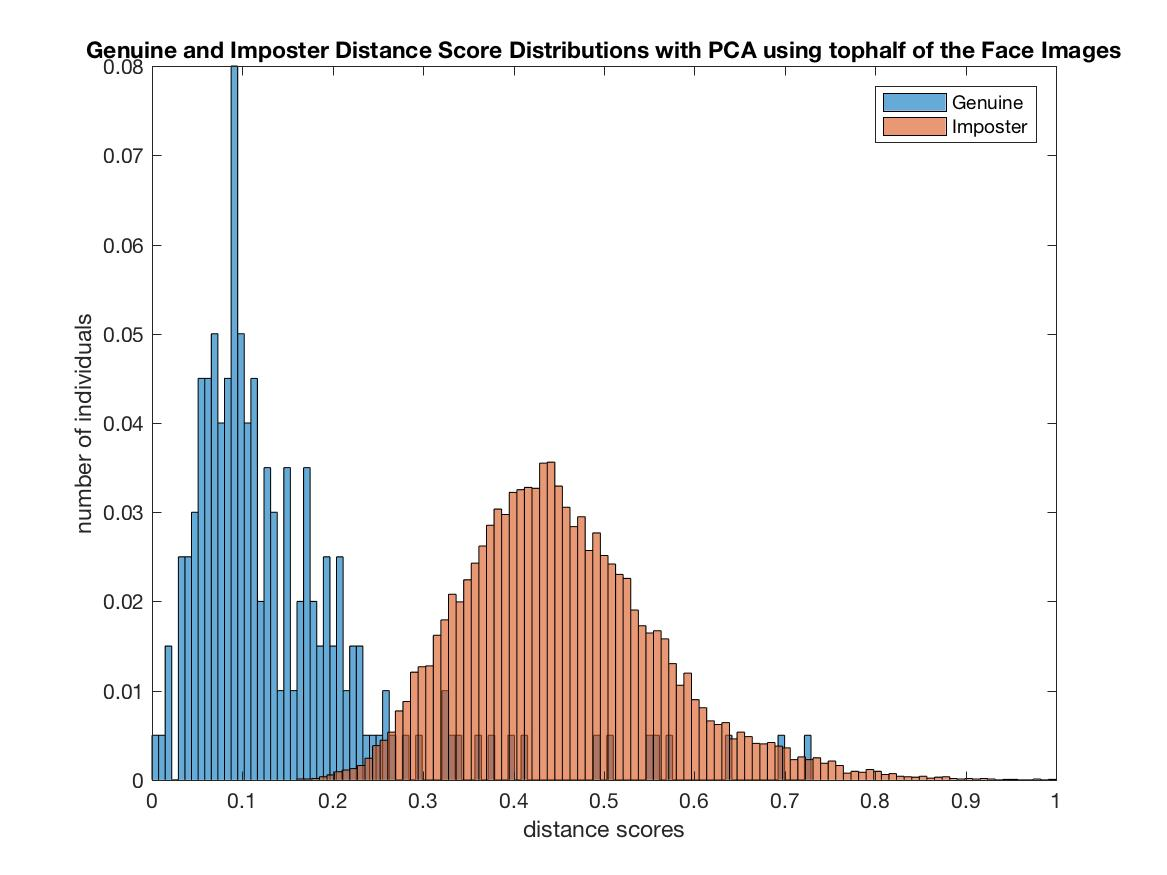
\includegraphics[width = 3.5in]{pcatopscoreDis.jpg}
	\caption{The genuine and imposter score distributions when only top half of the facial images are used.}
	\label{scoreDisTopPCA}
	\end{minipage}
	\begin{minipage}[t]{0.5\linewidth}
	\centering
	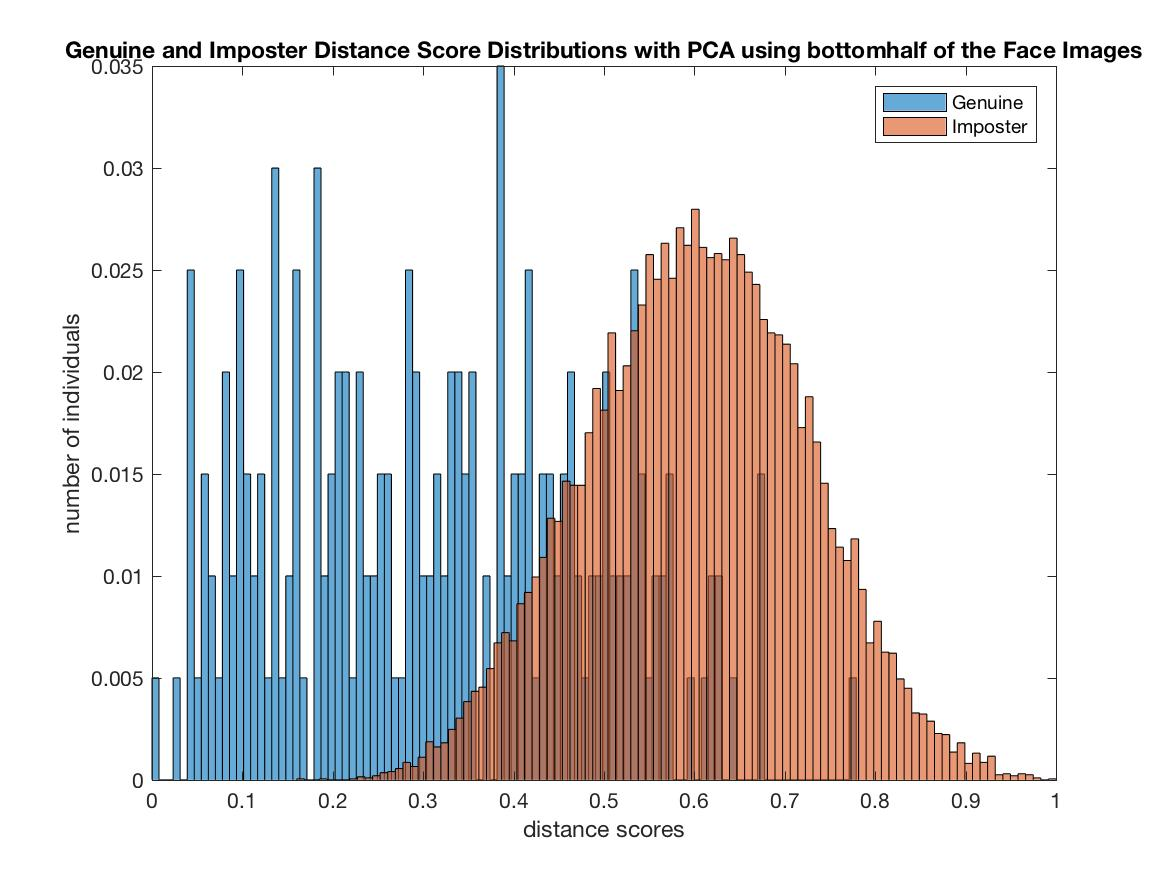
\includegraphics[width = 3.5in]{pcabottomscoreDis.jpg}
	\caption{The genuine and imposter score distributions when only bottom half of the facial images are used.}
	\label{scoreDisBottomPCA}
	\end{minipage}
	\end{figure}	
	
	\begin{figure}[h!]
	\begin{minipage}[t]{0.5\linewidth}
	\centering
	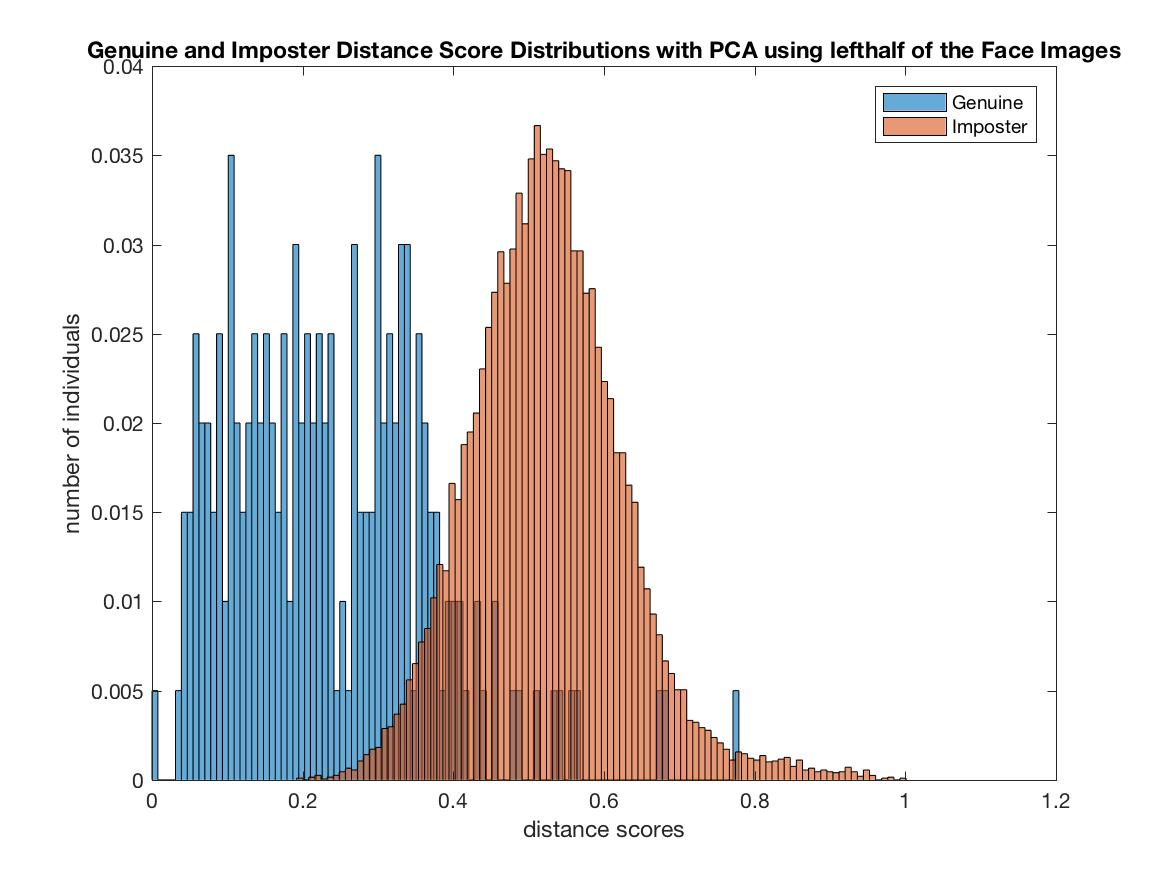
\includegraphics[width = 3.5in]{pcaleftscoreDis.jpg}
	\caption{The genuine and imposter score distributions when only left half of the facial images are used.}
	\label{scoreDisLeftPCA}
	\end{minipage}
	\begin{minipage}[t]{0.5\linewidth}
	\centering
	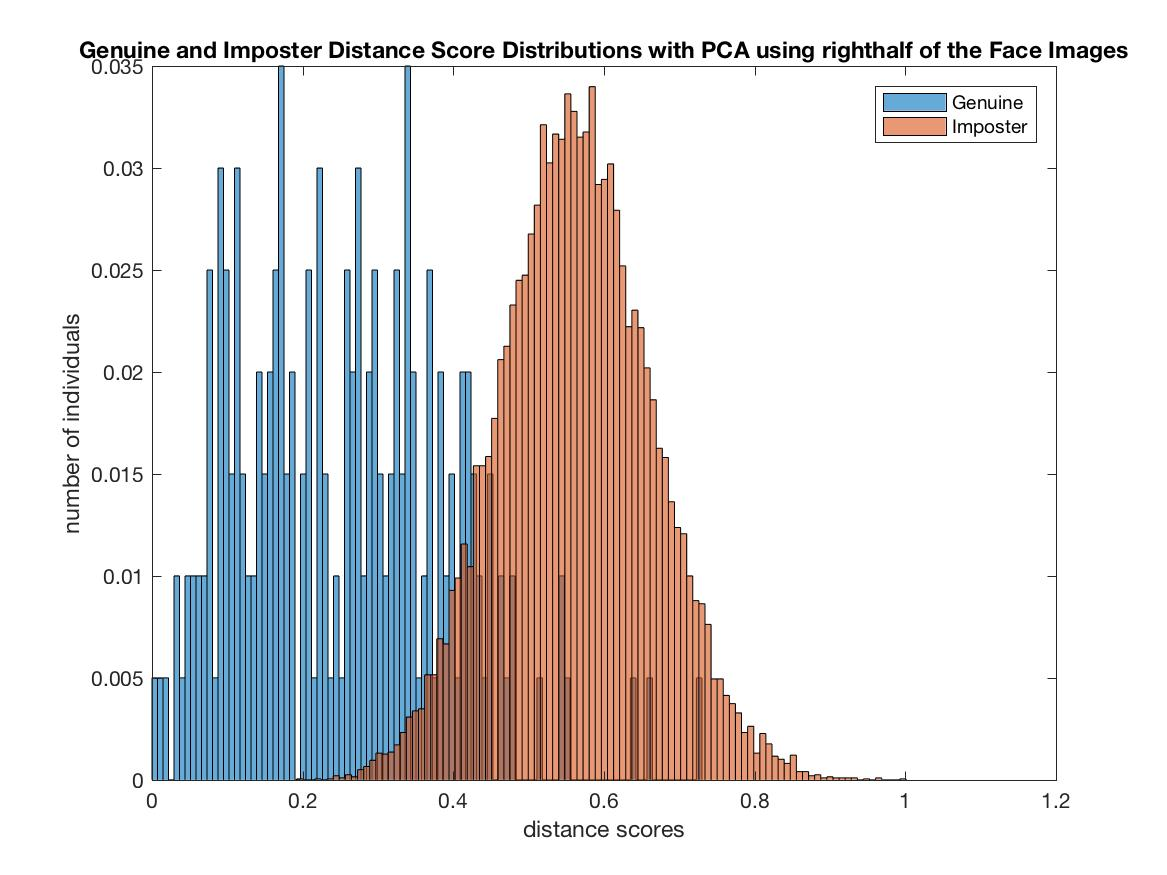
\includegraphics[width = 3.5in]{pcarightscoreDis.jpg}
	\caption{The genuine and imposter score distributions when only right half of the facial images are used.}
	\label{scoreDisRightPCA}
	\end{minipage}
	\end{figure}
	
	\begin{figure}[h]
	\begin{minipage}[t]{0.5\linewidth}
	\centering
	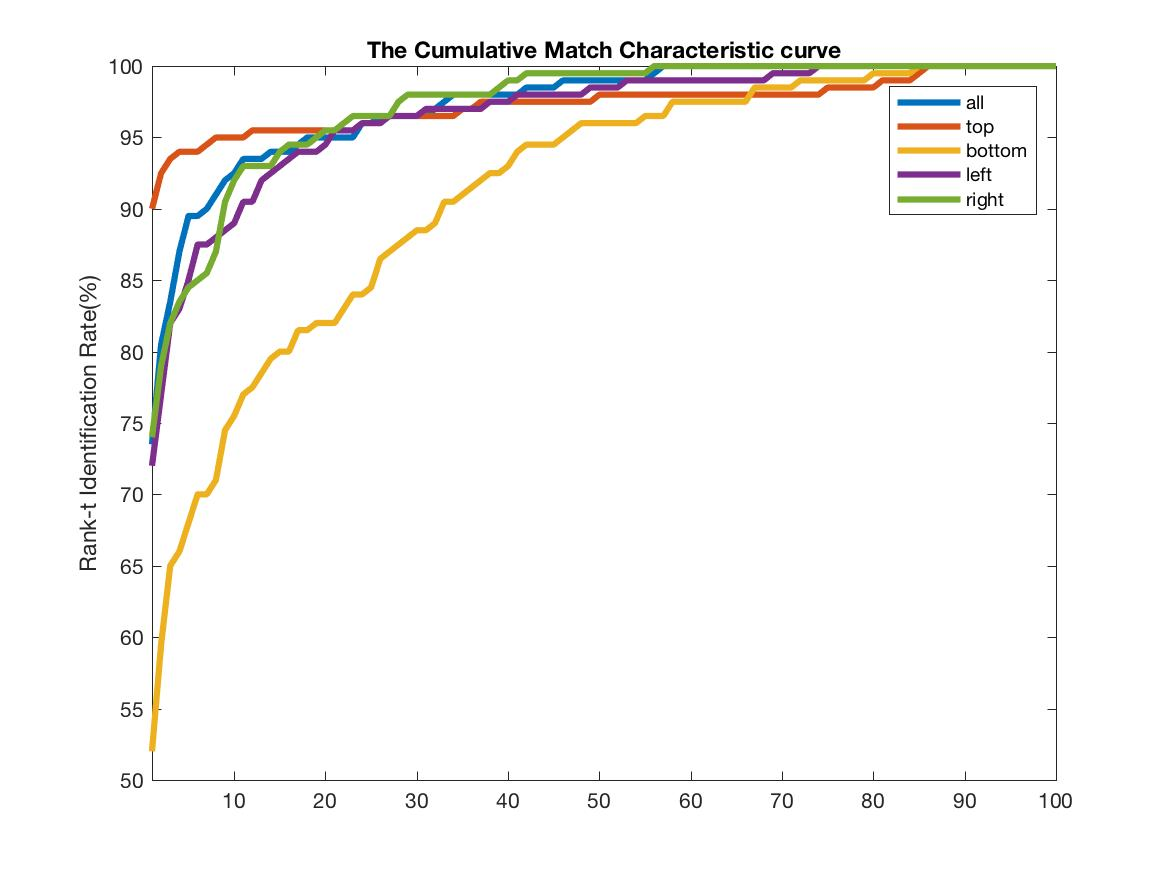
\includegraphics[width = 3.5in]{PCAinoneCMC.jpg}
	\caption{The comparison of the Cumulative Match Characteristic curve when using whole face, top, bottom, left and right half of the face images, when PCA is used to reduce dimensionality.}
	\label{cmcComPCA}
	\end{minipage}
	\begin{minipage}[t]{0.5\linewidth}
	\centering
	\includegraphics[width = 3.5in]{PCAinoneROC.jpg}
	\caption{The comparison of the Receiver Operating Characteristic curve when using whole face, top, bottom, left and right half of the face images, when PCA is used to reduce dimensionality.}
	\label{rocComPCA}
	\end{minipage}
	\end{figure}
	
	\begin{table}[h]
	\centering  
	\begin{tabular}{lccc}  
	\hline
	Part of face image & $d'$ value & rank-1 identification rate & rank-10 identification rate\\ \hline  
	entire & 2.5833 & $73.5\%$ & $92.5\%$\\         
	top & 2.6845 & $90.0\%$ & $95.0\%$\\      
	bottom &1.9053 & $52.0\%$ & $75.5\%$\\ 
	left &2.3951 & $72.0\%$ & $89.0\%$\\ 
	right &2.5634 & $74.0\%$ & $92.0\%$\\ \hline
	\end{tabular}
	\caption{Comparison of some performance measures}
	\label{comTablePCA}
	\end{table}
	
	Based on the plots and table shown above, we can see that with dimensionality reduced using principal component analysis, the result still says that with top half the face images being used, the performance is best. Several comments should be stated here: compared the former results whose similarity is measured using correlation coefficient, this result is obtained using Euclidean distance, which means, the larger the value, the less similar of the two objects being measured. What is more, as is known to all, the dimensionality reduction means the loss of information, while in this case, the result using eigenfaces does not seem worse than using all faces. Using principal component analysis actually means to project the faces in current space to the space of the eigenface, performance would not be improved by projection, thus the results would agree with those obtained using correlation based facial recognition.

	
	
	%\newpage
	%\large{Attached are code for part \uppercase\expandafter{\romannumeral1} :}
	%\normalsize
	%\begin{lstlisting}
	
	%\end{lstlisting}
	
	%\newpage
	%\large{Attached are code for part \uppercase\expandafter{\romannumeral2} }:
	%\normalsize
	%\begin{lstlisting}
	
	%\end{lstlisting}

	
\end{spacing}
\end{document}